\documentclass[a4paper,11pt]{article}
\usepackage{amsmath,amsthm,amsfonts,amssymb,amscd,amstext,vmargin,graphics,graphicx,tabularx,multicol} 
\usepackage[francais]{babel}
\usepackage[utf8]{inputenc}  
\usepackage[T1]{fontenc} 
\usepackage{pstricks-add,tikz,tkz-tab,variations}
\usepackage[autolanguage,np]{numprint} 

\setmarginsrb{1.5cm}{0.5cm}{1cm}{0.5cm}{0cm}{0cm}{0cm}{0cm} %Gauche, haut, droite, haut
\newcounter{numexo}
\newcommand{\exo}[1]{\stepcounter{numexo}\noindent{\bf Exercice~\thenumexo} : \marginpar{\hfill /#1}}
\reversemarginpar


\newcounter{enumtabi}
\newcounter{enumtaba}
\newcommand{\q}{\stepcounter{enumtabi} \theenumtabi.  }
\newcommand{\qa}{\stepcounter{enumtaba} (\alph{enumtaba}) }
\newcommand{\initq}{\setcounter{enumtabi}{0}}
\newcommand{\initqa}{\setcounter{enumtaba}{0}}

\newcommand{\be}{\begin{enumerate}}
\newcommand{\ee}{\end{enumerate}}
\newcommand{\bi}{\begin{itemize}}
\newcommand{\ei}{\end{itemize}}
\newcommand{\bp}{\begin{pspicture*}}
\newcommand{\ep}{\end{pspicture*}}
\newcommand{\bt}{\begin{tabular}}
\newcommand{\et}{\end{tabular}}
\renewcommand{\tabularxcolumn}[1]{>{\centering}m{#1}} %(colonne m{} centrée, au lieu de p par défault) 
\newcommand{\tnl}{\tabularnewline}

\newcommand{\trait}{\noindent \rule{\linewidth}{0.2mm}}
\newcommand{\hs}[1]{\hspace{#1}}
\newcommand{\vs}[1]{\vspace{#1}}

\newcommand{\N}{\mathbb{N}}
\newcommand{\Z}{\mathbb{Z}}
\newcommand{\R}{\mathbb{R}}
\newcommand{\C}{\mathbb{C}}
\newcommand{\Dcal}{\mathcal{D}}
\newcommand{\Ccal}{\mathcal{C}}
\newcommand{\mc}{\mathcal}

\newcommand{\vect}[1]{\overrightarrow{#1}}
\newcommand{\ds}{\displaystyle}
\newcommand{\eq}{\quad \Leftrightarrow \quad}
\newcommand{\vecti}{\vec{\imath}}
\newcommand{\vectj}{\vec{\jmath}}
\newcommand{\Oij}{(O;\vec{\imath}, \vec{\jmath})}
\newcommand{\OIJ}{(O;I,J)}

\newcommand{\bmul}[1]{\begin{multicols}{#1}}
\newcommand{\emul}{\end{multicols}}

\newcommand{\reponse}[1][1]{%
\multido{}{#1}{\makebox[\linewidth]{\rule[0pt]{0pt}{20pt}\dotfill}
}}

\newcommand{\titre}[5] 
% #1: titre #2: haut gauche #3: bas gauche #4: haut droite #5: bas droite
{
\noindent #2 \hfill #4 \\
#3 \hfill #5

\vspace{-1.6cm}

\begin{center}\rule{6cm}{0.5mm}\end{center}
\vspace{0.2cm}
\begin{center}{\large{\textbf{#1}}}\end{center}
\begin{center}\rule{6cm}{0.5mm}\end{center}
}



\begin{document}
\pagestyle{empty}
\titre{Interrogation: Nombres relatifs}{Nom :}{Prénom :}{Classe}{Date}



\exo{2} Cours :\\

\q Comment appelle-t-on l'ensemble des nombres positifs et négatifs ? \\
\reponse[1]\\

\q Donner la définition de l'opposé d'un nombre.\\
\reponse[2]\\

\q Déterminer l'opposé de chacun des nombres suivants :
-8,1 ;  123 ;  0 ;  -0,004\\
\reponse[1]\\

\q Quel est l'opposé de l'opposé de l'opposé de 4,8 ?\reponse[1]\\

\exo{3}\\

\initq 
\q Sur une droite graduée, placer :

\qa les points D, E et S d'abscisses respectives 4 ; -2 et -5,5,

\qa le point D' dont l'abscisse est l'opposée de celle du point D,

\qa le point E' dont l'abscisse est l'opposée de celle du point E.\\

\vspace*{3cm}




\q Que peut-on dire des points : D et D'?   E et E'?\\
\reponse[1]\\

\exo{3} 

\bmul{2}

\initq \q Compléter les phrases suivantes :
\bi
\item O est .................... du repère,  O a pour abscisse .... et  pour ordonnée ...... .

\item D  a  pour  coordonnées D(... ; ...).

\ei

\columnbreak

\begin{center}
\includegraphics[scale=1]{interro.eps} 
\end{center}

\emul

\q Placer dans le repère les points suivants : K(-4 ; 0) et V(-1 ; 3). \\

\newpage

\exo{2}

\initq
\q Ranger dans l'ordre décroissant les nombres : -1,64  ;  -1,6  ;  -1,69  ;  -1,7  ;  -1,66.\\
\reponse[1]\\

\q Compléter avec les signes <, > ou = :\\

\bmul{4}
     
   –18 ...... –9 
   \columnbreak
   
  -0,5 ...... 0
  
  \columnbreak
      
  –1,99 ...... –1,999 
  
  \columnbreak
  
   -10,010 ...... –10,01         

\emul



\end{document}
